\documentclass[a4paper,12pt]{article}
\usepackage{graphicx}
\usepackage{eso-pic}
\usepackage[utf8]{inputenc}
\usepackage[T1]{fontenc}
\usepackage[french]{babel}

\usepackage[colorlinks=True,citecolor=black,urlcolor=blue,linkcolor=black]{hyperref}
\usepackage{subfigure}
\usepackage[francais]{layout}
\usepackage{color}
\usepackage[table]{xcolor}
\usepackage{listings}
\usepackage{fancyhdr}
\lstset{
aboveskip=3mm,
belowskip=-2mm,
backgroundcolor=\color{darkWhite},
basicstyle=\footnotesize,
breakatwhitespace=false,
breaklines=true,
captionpos=b,
commentstyle=\color{red},
deletekeywords={...},
escapeinside={\%*}{*)},
extendedchars=true,
framexleftmargin=16pt,
framextopmargin=3pt,
framexbottommargin=6pt,
frame=tb,
keepspaces=true,
keywordstyle=\color{blue},
language=C,morekeywords={*,...},
numbers=left,
numbersep=10pt,
numberstyle=\tiny\color{black},
rulecolor=\color{black},
showspaces=false,
showstringspaces=false,
showtabs=false,
stepnumber=1,
stringstyle=\color{gray},
tabsize=4,
title=\lstname,
}


\usepackage[utf8]{inputenc}
\title{Projet jeu Darkest Dungeon}
\author{\textsc{Monjoux} Hugo & \textsc{Rivière} Hadrien & Option IS TP1}
\date{18 Septembre 2018}
\usepackage[a4paper,top=1.5cm,bottom=1.5cm,left=1.5cm,right=1.5cm,marginparwidth=1.75cm]{geometry}

\pagestyle{fancy}
\fancyhf{}
\chead{MONJOUX Hugo | RIVIERE Hadrien | Rendu 1.final | Page \thepage}

\begin{document}
\maketitle
\begin{figure}[!ht]
  \centering
  \includegraphics[width=1\textwidth]{Rendu1.1/ecran_acceuil.jpg}
  \caption{Aperçu du jeu "The Darkest Dungeon"}
\end{figure}

\newpage
\tableofcontents
\newpage
\section{Présentation Générale}
\subsection{Archétype}
Notre jeu s'inspire de Darkest Dungeon, qui est un RPG tour par tour, Rogue-like. Ce jeu est illustré dans les différentes figures exposées en fin du rapport. 

\subsection{Règles du jeu}

 Ce dernier permet au joueur d'évoluer soit en tant que héros, soit en tant qu'ennemis. L'objectif du joueur varie donc selon ce choix fait en début de partie. Si le joueur choisit de jouer en tant que héros, il doit arriver à la fin du niveau. Dans l'autre cas le joueur doit s'assurer que les héros n'arrive pas à la fin du niveau. 
\\ 
\indent
Le jeu se compose en trois vues : 
\begin{itemize}
    \item Vue d'accueil du joueur, qui pourra définir son équipe de héros, ainsi que l'inventaire de l'équipe, soit la répartition des ennemis sur les cartes de jeu
    \item Vue de déplacement dans le donjon
    \item Vue de combat lors de la confrontation des héros avec les ennemis
\end{itemize} 
\subsection{Ressources}
\begin{figure}[!ht]
  \centering
  \includegraphics[width=0.8\textwidth]{Rendu1.1/background3.jpg}
  \caption{Premier élément de décor : couloir}
\end{figure}
\begin{figure}[!ht]
  \centering
  \includegraphics[width=0.8\textwidth]{Rendu1.1/background4.jpg}
  \caption{Deuxième élément de décor : salle}
\end{figure}
\begin{figure}[!ht]
  \centering
  \includegraphics[width=1\textwidth]{Rendu1.1/ecran_acceuil.png}
  \caption{Ecran d'accueil avec à l'intérieur du cadre, le menu d'accueil (New game, Options...)}
\end{figure}
\begin{figure}[!ht]
  \centering
  \includegraphics[width=0.6\textwidth]{Rendu1.1/pers_licantrope.png}
  \caption{Exemple de design d'un personnage se transformant. Seulement les sprites encadrés seront utilisés pour alléger les ressources.}
\end{figure}
\begin{figure}[!ht]
  \centering
  \includegraphics[width=1\textwidth]{Rendu1.1/city1.png}
  \caption{Ville d'accueil du joueur avec de gauche à droite encadrés :  Auberge de recrutement pour modifier l'équipe, Sauvegarde de la progression, et Magasin pour remplir l'inventaire de l'équipe.}
\end{figure}
\begin{figure}[!ht]
  \centering
  \includegraphics[width=1\textwidth]{Rendu1.1/combat.png}
  \caption{Ecran de jeu principal : encadrés en gris clair, les héros à gauche et les ennemis à droite avec leur barre de vie respectives situées en dessous | encadrés en orange, les différents outils à dispositions du joueur (compétences, statistiques des personnages, équipements, carte, inventaire). Ces éléments seront adaptés aux contraintes de temps et de moyens de notre projet.}
\end{figure}
\clearpage
\newpage
\section{Description et conception des états}
\subsection{Description des états}
La partie, une fois le jeu lancée, est caractérisée par la paramétrisation du joueur et sa customisation de celle-ci lors de l'outgame. Notamment, le choix héros/ennemis évoqué ci-haut, la sauvegarde ou l'accès à un magasin pour remplir l'inventaire. 
\\ \indent
Puis une fois dans la partie ingame, l'état de jeu est formé par les éléments fixes (cartes, éléments de gameplay, ressources graphiques...) et des éléments mobiles (héros, ennemis, barres de vie, ordering lors des combats...). Les éléments mobiles dits vivants (héros et ennemis) sont répérés par une position sur une liste de salles existantes sur le donjon en cours d'exploration. 

\subsubsection{Etat éléments fixes}
Les différentes cartes, à l'instar de celles trouvables en FIGURE 6 et en bas à droite de la FIGURE 7, sont des cartes statiques présentant des ressources graphiques majoritairement statiques. L'ensemble de ces éléments ne seront intéractifs que par des effets de surbrillance ou d'ombre. 
\\ \indent
La \textbf{première carte illustrée en FIGURE 6} caractérisant la classe Village sert d'accueil au joueur souhaitant jouer côté Héros, et présentent un carrefour entre l'Auberge (constitution de l'équipe), l'Eglise (Sauvegarde), le Magasin (acheter des items pour l'inventaire de l'équipe), et le Carrosse (partir à la conquête des donjons). Sur cette carte on retrouve : 
\begin{itemize}
    \item Le Village : qui donne accès à la fois au Carrosse ainsi qu'à l'Eglise
    \item L'Auberge : qui donne accès à la customisation de l'équipe.
    \item Le Magasin : qui donne accès à un autre écran sur lequel le joueur peut acheter des items (Potions et autres items détaillés plus tard).
    \item Les Item : un listing des items obtenables par le Shop afin d'équiper le joueur au sein du Donjon, caractérisés par des méthodes singulières selon la nature de l'item.
    \item Le Donjon : un listing de toutes les salles, ainsi que leur composition, ainsi que la position du joueur
    \item Les Rooms : des instances qui réunissent à la fois la team ainsi que les différents ennemis
\end{itemize}
\\ \indent
La \textbf{deuxième carte illustrée en FIGURE 7 en bas à droite} permet au joueur de se déplacer dans le donjon dans lequel il progresse. Cette carte intègre une unique ressource graphique qui est faite à la main, représentant le plan du donjon. Les salles, indiquées par des carrés, seront associées à des phéonomènes de surbrillance par exemple si le joueur s'y déplace.



\subsubsection{Etat élements mobiles}
Les éléments mobiles possèdent une position de départ qui correspond à leur position sur l'écran de combat avant que l'attaque soit effectuée. Ils ont ensuite une vitesse de déplacement qui correspond à la vitesse à la quelle le sprite se déplace sur l'écran. 

\begin{itemize}
\item Personnages (héros ou monstres): Ces éléments sont controllés soit par un humain soit par une IA. Leur mouvement correspondent aux choix faits par l'un d'entre eux. Les actions qui s'en suivent sont associées à ces choix mais sont prédéfinies dans le jeu (charge lors de l'attaque au corps à corps, personnage tremble après avoir reçu un coup, utilisation des skills...).
\item Icônes de personnages : ces icônes qui se situent en haut de l'écran de combat se déplacent en fonction du tour. Celle la plus à gauche correspond au personnage qui joue le plus tôt.
\end{itemize}
\newpage
\subsubsection{Etats généraux}
L'ensemble de ces états sont complétés par un état général qui résume l'état du jeu comme défini ci-dessous à un instant t : 
\begin{itemize}
    \item Une horloge permettant de rythmer les tours de jeu en ingame, ainsi que l'apparition et la désapparition des éléments in et outgame. 
    \item Le Gameplay du Game + est basé sur l'édition du nombre de donjons finis,
et du nombre de donjons finis successivement. Ainsi des conditionnelles sur ces chiffres peuvent être implémentées pour maximiser la durée de vie du jeu, ou simplement permettre de suivre le scoring du joueur sur sa partie. 
    \item L'Etat de l'équipe : la santé in-dungeon, l'état du personnage (en forme, en état de choc, empoisonné, mort...)
    \item L'état des salles du donjon visitées : la liste des salles, leur occupation (nombre de monstres, quels monstres), leur état (finies, non finies, où le héros se situe).
    \item L'inventaire : il s'agit de lister l'ensemble des item qui à un moment t appartiennent au joueur. 
Il est à noter que la sauvegarde, comme évoqué plus haut en section 2.1.1, conserve les deux premiers tirets de ces états généraux. 
\end{itemize}

\subsection{Conception logicielle}
Le diagramme de classe est présenté ci-dessous en FIGURE 8 et nous pouvons y observer plusieurs groupes de classes: 
\begin{itemize}
    \item \textbf{Classes Elements :} ces classes sont représentées en jaune sur le diagramme pour les classes intermédiaires, les classes objets finales (qui n'ont pas de filles) sont représentées en bleue, et caractérisent des archétypes (d'item, de personnages ou d'ennemis). Afin d'identifier les natures des classes des méthodes sont définies telles que, notamment si l'objet créé est un élément mobile ou statique, par des méthodes isStatic(), ou au sein de l'architecture des classes statiques, pour savoir si l'objet créé est un bâtiment avec une méthode isBuilding(). 
    \item \textbf{Conteneurs d'élement :} en vert, les classes State, ElementTab, Inventaire et Team qui permettent d'accumuler les éléments utiles à la partie du joueur. Les trois classes Inventaire, Team et ElementTab sont des conteneurs d'objets qui sont à dimensions finies (des tableaux de dimensions N éléments), et la classe State qui nous permet d'accéder à toutes les données de l'état du jeu à un instant donné. 
    \item \textbf{Observateurs de changements d'état} Ces classes sont représentées en mauves sur le dia : elles nous permettent de détecter un changement d'état, qui est ensuite notifier jusqu'à la Scene appartenant au dia du Render. Afin de déterminer les éléments visuels associés à cette modification et leur nature qui est analysée par le biais de Event. La conception de cette outil est basé sur le pattern Observer. 
\end{itemize}

\begin{figure}[!ht]
  \centering
  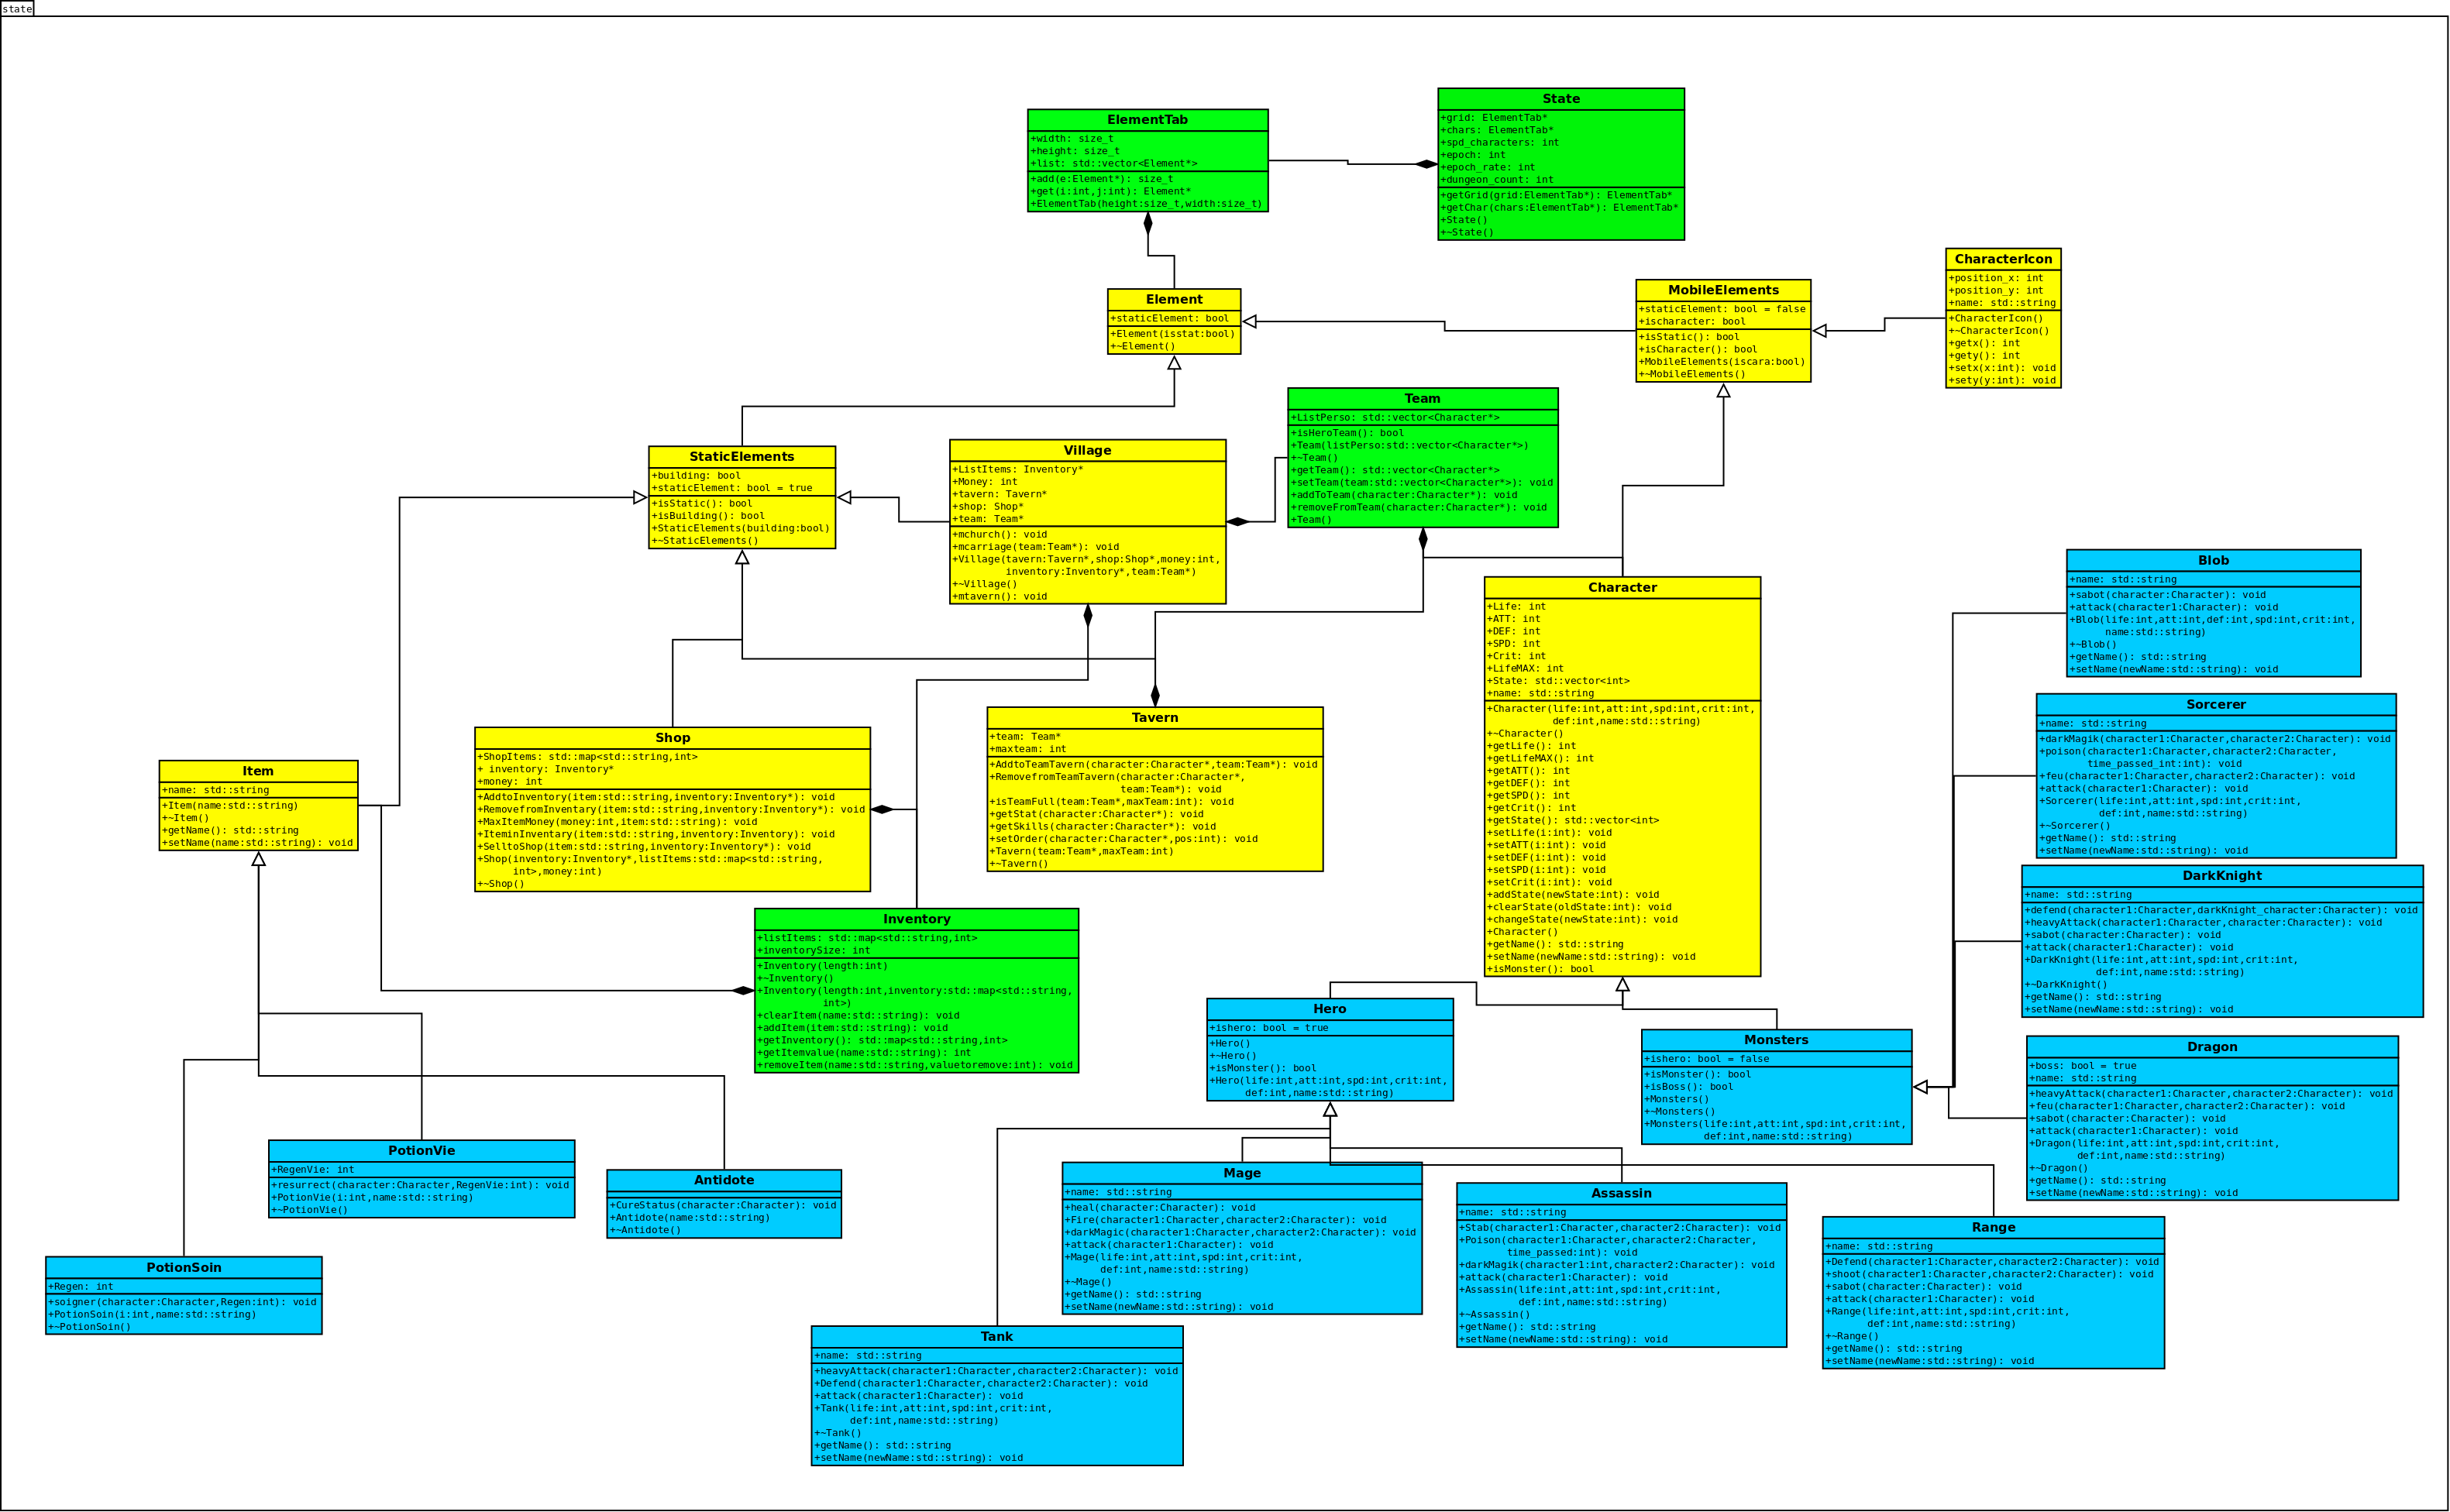
\includegraphics[angle=90,width=0.9\textwidth]{Rendu2.2/state.png}
  \caption{Diagramme de classe associé au projet fait via DIA}
\end{figure}
\clearpage
\newpage
\section{Rendu: Stratégie et conception}
\subsection{Stratégie de rendu d'un état}
La stratégie d'affichage du rendu se dirige vers un fonctionnement organisé en layers (calques) : ces derniers représentent chacun un plan. 
\\ \indent Chacun des plans est lui-même constitué des éléments provenants du diagramme state.dia affiché ci-dessus. Afin d'ordonner ces plans de manière optimale, il est nécessaire de les organiser de la sorte :
\begin{enumerate}
    \item Backgrounds : l'ensemble des éléments de décors intervenant sur l'arrière de l'écran (texture des salles, maps, ville, écran d'accueil...)
    \item Mobiles objects : l'ensemble des objets qui sont assimilés à une interactivité avec le joueur ou l'horloge interne du jeu (sprites en mouvement, bouton cliquable...)
    \item Effets : cela inclut tous les éléments graphiques ayant une signification à la fois dans l'aide de l'affichage, ou d'effet temporaires régis par une horloge (sprite attaques, halos lumineux ...) 
\end{enumerate}
\\
\\ \indent Chacun de ses plans contient à la fois les éléments placés sur une matrice (de dimensions le nombre de pixels en largeur et hauteur, ce qui sera probablement 2130x1440px) qui modélise une grille placée sur notre fenêtre d'affichage, ainsi qu'une texture à afficher selon le plan concerné. 
\\ \indent Les différentes couches de layers mettent notamment en évidence des changements d'états à la fois permanents, cycliques et temporaires. La plupart de ceux-ci sont donc gérés différemment mais temporiser par l'horloge interne difinie. 
\begin{itemize}
    \item Si le changement d'état donne lieu à l'édition du rendu de manière permanente : la matrice de plan est éditée notamment les couches basses (backgrounds)
    \item Si le changement d'état donne lieu à l'édition du rendu de manière temporaire : la matrice de plan est éditée et régulièrement mise à jour notamment les couches hautes (Mobiles objects et Effets)
\end{itemize}
Concernant la synchronisation, il faut distinguer deux fréquences d'édition :
\begin{enumerate}
    \item Une horloge étant associée à l'édition des états des éléments du jeu : celles-ci doit être relativement lente (de l'ordre de 0.1 s afin d'éditer plusieurs états par frame. Cependant elle doit être plus lente que l'horloge d'édition du rendu purement graphique.
    \item Une horloge associée au rendu graphique (mouvement des sprites, déplacement des personnages, déplacements des animations...) : celle-ci à l'instar de beaucoup de jeux-vidéo actuels, doit à minima tenir une cadence de 30Hz voir 60Hz si le rendu n'est pas trop lourd. 
\end{enumerate}
Concernant la gestion des rendus associés aux différentes horloges :
\begin{itemize}

    \item Certaines animations cycliques (mouvement des personnes, des ennemis, animations indiquant l'empoisonnement des personnages, halos lumineux sur des cases) disposeront de fréquences uniques leur étant associées, afin d'optimiser le rendu graphique.
    \item Les animations qui seront dépendantes de l'horloge d'état sont affichées selon des calculs de trajectoires selon leur définition unique. Par exemple si l'état d'un personnage X change vers la position d'attaque, alors le sprite (l'animation) de l'attaque suit une trajectoire partant du point de départ vers le point d'arrivée, sleon une certaine vitesses. Ensuite l'horloge de rendu graphique permettra d'afficher cette animation selon sa position en temps réel sur la matrice du rendu. 
\end{itemize}

\subsection{Conception logiciel}
Le diagramme de classe concernant le rendu global est présenté ci-dessous en FIGURE 9. Notre projet inclut des affichages statiques non composés de tuiles reproductibles, ce qui nous permet d'imaginer un diagramme de classe relativement simple, bien que designer de sorte à satisfaire plusieurs états d'affichages. Ce diagramme de classe est composé de : 
\newpage
\begin{itemize}
    \item Layers : la classe Layers instancie les différents plans constituant le rendu global. Cela constitue l'ensemble des informations envoyées à la carte graphique. Cette classe communique avec les Surfaces d'un côté, et les définitions de layers, associés soit à l'état de jeu, soit aux éléments constituants les états à un instant précis. 
    \\ Une fois la texture chargée, il faut donc structurer l'affichage à l'écran, qui est géré par la méthode de setSpriteLocation(), et setSpriteTexture(list), qui dans notre cas nous permet de gérer l'affichage structurer de chaque état. 
    \item Surface : Chaque surface est constituée d'une texture qui regroupe à elle-seule plusieurs sprites. Ces derniers représentent des types de ressources graphiques différentes (monstres, backgrounds, icônes, effets...) et sont concaténés dans cette texture. Chaque élément est placé selon le type d'état qui est défini dans l'état général, et les coordonnées de départ (en haut à gauche) et d'arrivée (en bas à droite) de chaque sprite.
    \item XDisplay : ces classes permettent de caractériser un display particulier associé à chacun des état du jeu. Nous en définissons ici 4 pour s'adapter à la majorité des états pour l'instant imaginés. Il est à noter que l'identité de l'état est récupéré par l'intermédiaire de state et nous permet d'identifier l'état à display. Par exemple pour l'état de combat défini par l'état Room, l'affichage et constant et demande N sprites avec des positions pré-définies dans les sous-classes évoquées.
\end{itemize}
Pour l'instant, par manque de temps, l'affichage est codé en dur, mais l'implémentation se poursuit pour coller à la description faite ci-dessus. L'affichage des états Tavernes ainsi que Shop ne sont à ce jour pas encore visibles. 

\begin{figure}[!ht]
  \centering
  \includegraphics[angle=90,width=0.9\textwidth]{Rendu2.2/render.png}
  \caption{Diagramme de classe associé au rendu global fait via DIA}
\end{figure}
\clearpage
\newpage 
\section{Régles de changements d'états et moteur de jeu}
\subsection{Changements extérieurs}
Ces changements sont provoqués par la pression sur une touche du clavier du joueur ou de l'utilisation de la souris (clic) : 
\begin{itemize}
    \item A partir du Village, le joueur est dirigé vers le choix du donjon
    \item Choix du donjon sur deux niveaux "EngineTest" et "The End".
    \item Des boutons de retour ou d'accès d'un état : "Donjon", "Back"
    \item Durant les combats le choix des différentes skills cliquables par le joueur
    \item A chaque écran, les boutons de retour à l'écran précédent
\end{itemize}

\subsection{Changements autonomes}
Les changements autonomes sont exécutés en cascade à partir d'un changement extérieur. 
\begin{itemize}
    \item Une fois dans le room, la commande de calcul du personnage actif est effectuée automatiquement afin de déterminer l'ordre des personnages actifs qui joueront durant la partie
\end{itemize}

\subsection{Conception logiciel}
Le diagramme de classe du moteur est présenté en Figure 10, et nous présente l'implémentation que nous avons imaginé pour les différents changemets précédemment décrits.

\\ \indent Classe Command : le rôle de ces différents classes listées ci-dessous, est de caractériser un comportement à l'origine d'un changement de nature autonome, extérieur, ou système. Grâce au CommandTypeId, nous allons identifier chaque instance de Command créée, afin d'y associer son comportement : 
\begin{enumerate}
    \item BackCommand : retour sur la scène précédente
    \item CalculateActiveCommand : calcul du prochain personnage qui doit jouer lors du combat 
    \item ChooseDungeonCommand : choix du donjon par le joueur
    \item CreateDungeonCommand : création du donjon, lorsque le joueur provient du Village
    \item CreateRoomCommand : création de la salle de combat 
    \item CreateVillageCommand : création du Village
    \item UseSkillCommand : utilisation d'une attaque par le joueur lors d'un combat
\end{enumerate}

\\ \indent Classe Engine : cette classe est essentielle au bon fonctionnement de l'ensemble de la gestion des commandes. En effet, chaque commande est priorisée de manière unique. Cela permet à chaque époque, d'accumuler les différentes commandes à traiter dans un std::map, et de les exécuter selon leur ordre de priorité. Une fois les commandes exécutées, elles sont supprimées.

\begin{figure}[!ht]
  \centering
  \includegraphics[angle=90,width=0.9\textwidth]{Rendu2.2/engine.png}
  \caption{Diagramme de classe associé au moteur de jeu fait via DIA}
\end{figure}

\end{document}